The basic fact that fine-tuning can work for transfer learning is that Deep CNN can learn hierarchical features from bottom to top and some of the features are task-independent, especially most low-level and some mid-level ones.

There are two major strategies to fine-tune the deep CNNs: fine-tune the last layer (i.e. the classifier layer) and fine-tune the whole net.

\begin{itemize}
	\item \textbf{Fine-tune the last layer.} In the first strategy, we consider the deep CNNs as a fixed feature extractor and only modify the last layer of the net. This assumes that the features extracted by the pre-trained deep CNN can be directly applied to the new tasks. Therefore, by changing the last layer of the model, e.g. the combination of the features, the model can adopt new classes effectively. For example, when we introduce the mythical creature Sphinx to someone, we usually say it has the head of a human, the haunches of a lion, and the wings of a bird and people could obtain a rough idea of how Sphinx looks like without even see its picture. Here, the features such as head and haunches to describe Sphinx are high-level features that can be adopted directly from learned knowledge. Without learning from scratch, we can adopt the new concept effectively.
	\item \textbf{Fine-tune the while net.} When fine-tuning the whole net, typically, we assume that some of the features extracted from the pre-trained deep CNN are not good enough for the new tasks. Therefore, we have to learn some new high-level features again. In fact, the high-level features are task-dependent and can be learned from those task-independent low-level features with certain combination. The purpose of fine-tuning the whole net is to changing the combination of the low-level features to reconstruct the task-dependent high-level features for the new task. 
\end{itemize}

For both strategies, the last layer, i.e. the layer of a classifier is removed. For different fine-tuning strategies, the error would back propagate to different layers (see Figure \ref{fig:ft-net}). Typically, a small learning rate is used to for fine-tuning the model to make sure that the model will not overfit the data of the target task.

\begin{figure}
	\centering
	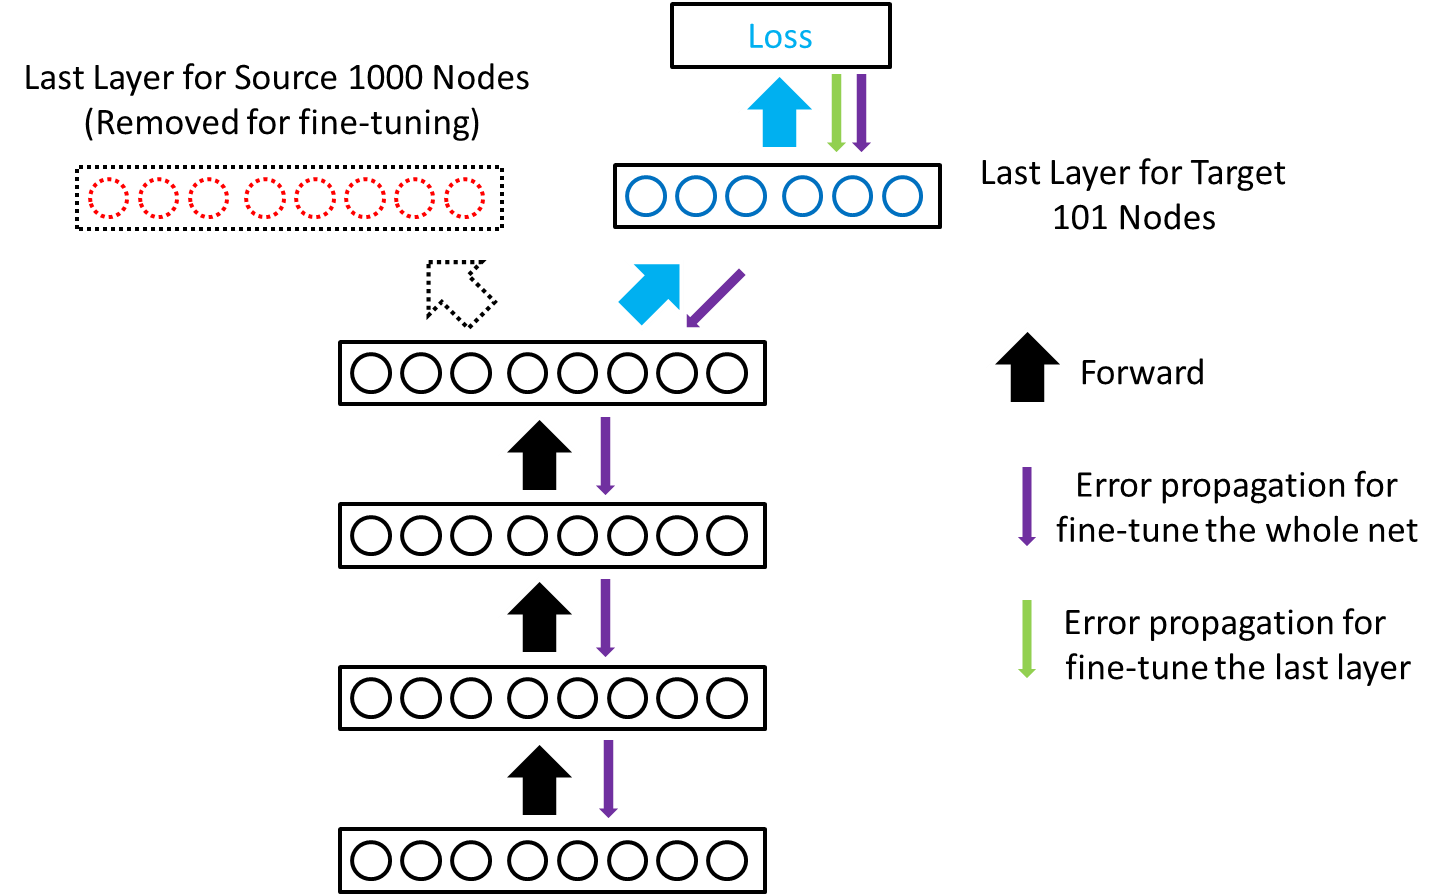
\includegraphics[scale=.5]{cnn/fig/ft.png}
	\caption{Demonstration of Fine-tuning from ImageNet 1000 classes to Food-101 datasets.}
	\label{fig:ft-net}
\end{figure}